\section{Experiments}\label{sec:experiments}
The experiments ask three questions about trained rules. \textbf{Q1:} what does pre-commitment cost when each class uses its best design? \textbf{Q2:} how much of that comparison is design optimization, and can the designs be found without knowing the population? \textbf{Q3:} what does a working model change, including when it is wrong? Every population $P$ is a held-out or target empirical law mixed with a uniform mass of $1\%$ over profiles and labels, which gives full support; every design-based score is pointwise unbiased; every constant is certified by primal and dual bounds that agree to a relative error of at most $10^{-4}$ ($10^{-3}$ within a model) unless a bound or an interval is shown. Protocols, per-run values and sensitivity analyses are in Appendix~\ref{app:F}.

\begin{table*}[t]
\centering
\caption{BRFSS screening trees on twelve items (six runs per cap: two targets, three seeds): records needed relative to a branching interview that asks the tree\textquotesingle s own questions (which attains the full-information variance); medians over the six runs, range in brackets. \emph{Pre-committed forms without a model} (pointwise-unbiased scores): the optimal design at the target law; the design fitted on 20,000 source records; the design learned from a cross-fitted pilot of the audit itself with smoothed cell masses, all records charged ($N=4{,}000$; 1 when one form holds all the rule\textquotesingle s items); uniform randomization over all forms of the rule\textquotesingle s items and over the tree\textquotesingle s question paths, each with optimal tables. \emph{Two rounds}: the optimal two-round design (at $b=6$ the median includes certified upper bounds from feasible two-round designs for 4 runs, Table~\ref{tab:runs}). \emph{Bracket}: $[1/\rho_P^2,\ N_P]$ of Theorem~\ref{thm:bracket}. \emph{Within a model}: $W^{(k)}_{\rm fixed}/W^{(k)}_{\rm branch}$ at the order-$k$ log-linear fit of the target law.}
\label{tab:screening}
\footnotesize
\setlength{\tabcolsep}{2.4pt}
\begin{tabular}{r l r r r r r l l l}
\toprule
 & \multicolumn{5}{c}{pre-committed forms, no model} & two & bracket & \multicolumn{2}{c}{forms within a log-linear model} \\
\cmidrule(lr){2-6}\cmidrule(lr){9-10}
$b$ & optimal & reference & pilot & uniform, items & uniform, paths & rounds & $[1/\rho_P^2,N_P]$ & pairwise & three-way \\
\midrule
3 & 1.00 [1.00, 1.34] & 1.04 & -- & 1.00 & 1.03 & 1.00 & [1.00, 1.5] & 1.00 [1.00, 1.09] & 1.00 [1.00, 1.23] \\
4 & 1.49 [1.00, 1.75] & 1.57 & 1.62 & 2.30 & 1.80 & 1.00 & [1.18, 3.3] & 1.09 [1.00, 1.13] & 1.28 [1.00, 1.40] \\
5 & 1.35 [1.18, 1.54] & 1.42 & 1.53 & 2.04 & 1.72 & 1.00 & [1.08, 5.4] & 1.06 [1.02, 1.10] & 1.17 [1.08, 1.28] \\
6 & 1.58 [1.42, 1.98] & 1.68 & 1.93 & 4.18 & 2.30 & $\le$1.05 & [1.13, 10.5] & 1.07 [1.05, 1.13] & $\ge$1.18 [1.15, 1.33] \\
\bottomrule
\end{tabular}
\end{table*}


\paragraph{Q1: the cost of pre-commitment.}
A depth-$b$ screening tree asks at most $b$ questions per person, so a validation study under the same burden must respect the cap. We train class-balanced CART trees on twelve yes/no items of the CDC Diabetes Health Indicators, derived from the Behavioral Risk Factor Surveillance System (BRFSS; 253,680 respondents, target diabetes or prediabetes) \citep{cdcdiabetes2017}, and on twelve binarized thyroid items \citep{quinlan1986thyroid}, and validate them on a disjoint random half or on respondents of the other sex. On thyroid, and whenever a tree uses at most $b$ items, one form asks everything the rule needs and pre-commitment costs nothing. On BRFSS at caps four to six the best pre-committed design needs a median \nScreenBestLo--\nScreenBestHi{} times the respondents of branching (\nScreenRunLo--\nScreenRunHi{} over runs; Table~\ref{tab:screening}); label-dependent form probabilities lower this by at most \nLabelMax\%. \nRulesSentence{} A second round removes most of the gap: of the \nScreenGainN{} BRFSS diabetes trees with a gain, \nGainComputable{} are computed exactly by a two-round interview, \nGainExactNon{} more are within a factor \nScreenTwoMax{} of branching, and the remaining \nTwoBounded, at $b=6$, within \nTwoBoundMax{} (Figure~\ref{fig:rounds}a).

\begin{table}[t]
\centering
\caption{Further rules (depth-$b$ trees, $b\in\{4,5,6\}$, three seeds; BRFSS outcomes on 21 variables, Spambase on 57 features): records needed relative to branching by optimal and by uniformly drawn forms on the rule\textquotesingle s items, median [range] over the runs with a gain. Runs: with a gain / without (the rule uses at most $b$ items) / not computed (more than 13 items, or not finished). Pairwise: $W^{(2)}_{\rm fixed}/W^{(2)}_{\rm branch}$ at the pairwise fit (rules with at most ten items). Details and bootstrap ranges: Table~\ref{tab:rules}.}
\label{tab:rulesmain}
\footnotesize
\setlength{\tabcolsep}{2pt}
\begin{tabular}{llllr}
\toprule
target & runs & optimal forms & uniform, items & pairw. \\
\midrule
heart disease & 7/0/2 & 1.57 [1.16, 2.38] & 3.2 [1.4, 16.8] & 1.16 \\
stroke & 6/0/3 & 1.34 [1.30, 1.79] & 2.1 [1.9, 3.7] & 1.12 \\
high blood pr. & 7/0/2 & 1.13 [1.07, 1.33] & 1.4 [1.3, 1.6] & 1.01 \\
diff. walking & 4/2/3 & 1.40 [1.24, 1.56] & 2.0 [1.4, 2.8] & 1.07 \\
spam & 4/0/5 & 1.97 [1.40, 2.06] & 4.8 [2.2, 8.4] & 1.18 \\
\bottomrule
\end{tabular}
\end{table}


\emph{Ensembles.} On WDBC, Spambase and Ionosphere \citep{wolberg1993,spambase1999,ionosphere1989}, an old and a new random forest of twenty depth-$b$ trees are trained on disjoint records with $m\in\{6,9,12\}$ median-binarized features; the contrast is the difference of the forests' predicted probabilities, which no single interview computes. At cap three the best pre-committed design needs a median \nCapThreeMed{} times the records of the best branching design (range \nCapThreeMin--\nCapThreeMax, Table~\ref{tab:capgrid}), and an optimal two-round design at most \nTwoForestRatioMax{} times in each of \nTwoForestN{} tasks. Here the cap costs more than pre-commitment: relative to complete records, the best fixed designs need \nCapFixLo--\nCapFixHi{} and the best branching designs \nCapBrLo--\nCapBrHi{} times as many (medians by cap). \nForestScaleSentence

\begin{figure}[t]
\centering
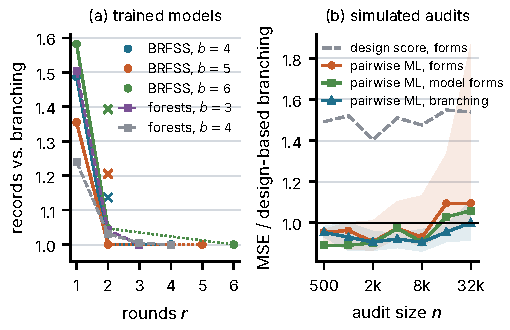
\includegraphics[width=\columnwidth]{figures/v19_rounds.pdf}
\caption{(a) Records needed relative to branching, without a model, as a function of the number of rounds ($r=1$: fixed forms; $r=b$: branching): optimal $r$-round designs for BRFSS screening trees (median over runs; at $b=6$, $r=2$ the median includes upper bounds) and forest updates (median over tasks); crosses mark the heuristic of following the root question. (b) Simulated audits: mean squared error relative to the design-based mean under branching, against the audit size, for the design-based form score and for pairwise maximum likelihood on fitted forms, on forms optimized for the pairwise model, and on branching records (median over \nCurveTrees{} BRFSS trees; bands: quartiles).}
\label{fig:rounds}
\end{figure}

\paragraph{Q2: design optimization versus adaptivity.}
The ratios above compare optimized designs, and optimization accounts for much of what a naive comparison would credit to adaptivity. Uniform randomization over all forms of the rule's own items, with optimal tables, needs a median \nUitMedLo--\nUitMedHi{} times the records of branching by cap, and uniform matrix sampling over all twelve items \nUnifLo--\nUnifHi{} times; uniform randomization over the tree's question paths needs a median \nUpsOverMed\% more than the optimized forms. The optimized designs do not require knowing the population. Forms fitted on 20,000 source records need a median \nFitMed\% more than the oracle and stay exactly unbiased. With no reference, the design is learned from a pilot of the audit itself, which must be charged: with a quarter of $N=4{,}000$ records as a cross-fitted pilot on the tree's paths and cell masses smoothed by a pairwise fit, the all-in price is a median \nPilotAllLo--\nPilotAllHi\% above the oracle of the same run (\nPilotEmpLo--\nPilotEmpHi\% with unsmoothed frequencies; Table~\ref{tab:pilotsmooth}). The bracket of Theorem~\ref{thm:bracket} is loose on these rules, a median factor \nLowUnder{} below and \nNpOver{} above the realized ratio, so the solver is needed.

\begin{table}[t]
\centering
\caption{Forest updates of depth $b$ under cap $b$ (WDBC, Spambase, Ionosphere; binding tasks). Fixed/branch: exact $W_{\rm fixed}/W_{\rm branch}$, median [minimum, maximum]. Fit: median excess of the ratio realized by designs optimized on training records over the exact ratio of the same task ($^\dagger$the 15 tasks with $m=12$). Own: share of the log-gap captured when branching may use only the forests\textquotesingle{} own trees. Two: exact optimal two-round design, $W_2/W_{\rm branch}$ ($^\ddagger$five splits per cell: 45 and 15 tasks; at $b=2$ two rounds are branching). Cap: $W_{\rm fixed}$ and $W_{\rm branch}$ relative to the full-information variance.}
\label{tab:capgrid}
\footnotesize
\setlength{\tabcolsep}{2.6pt}
\begin{tabular}{rrlrrrrr}
\toprule
 & & & & & & \multicolumn{2}{c}{Cap: /full} \\
$b$ & tasks & Fixed/branch & Fit & Own & Two & fixed & branch \\
\midrule
2 & 45 & 1.31 [1.12, 1.49] & +1\% & 49\% & 1 & 4.1 & 3.3 \\
3 & 180 & 1.51 [1.14, 1.85] & +2\%$^\dagger$ & 17\% & 1.04$^\ddagger$ & 3.5 & 2.3 \\
4 & 15 & 1.24 [1.13, 1.35] & +3\% & 26\% & 1.03$^\ddagger$ & 1.4 & 1.1 \\
\bottomrule
\end{tabular}
\end{table}


\paragraph{Q3: what a working model changes.}
\emph{Constants when the model holds.} We refit each target law by the pairwise and the three-way log-linear model on the label and the rule's items and compute $W^{(k)}$ for forms and for depth-$b$ trees at the fit (\nModelRuns{} runs in which the rule depends on more than $b$ items; Table~\ref{tab:model}). Under the pairwise model pre-committed forms need \nModelTwoLo--\nModelTwoHi{} times the records of the best branching design, where the design-based ratio at the same laws is \nModelDesignLo--\nModelDesignHi; under the three-way model the ratio is \nModelThreeLo--\nModelThreeHi. The radius in part (b) of Theorem~\ref{thm:structured} is not explicit, so the theorem does not predict these values; they are computed. On synthetic laws the solver reproduces both ends of the theorem: at pairwise fits of noisy address populations the pairwise ratio stays at \nDepFitTwoMax, whereas along the strongly coupled laws of part (d) it rises from one to \nDepRatioLast{} at $b=3$ (Table~\ref{tab:dependence}).

\emph{When the model is wrong.} \nMisspecSentence

\emph{Simulated audits.} \nAuditParagraph

\paragraph{Further checks.}
An optimized design is tailored to one rule: scoring another tree on its records needs \nReuseMin{} to \nReuseMax{} times the records of branching, whereas one design shared by three known trees costs each a median \nJointPenMed\% more than its own optimum (Appendix~\ref{app:reuse}); the fixed optimum for all 21 BRFSS variables is certified in \nScaleMin{} minutes (Appendix~\ref{app:scale}). Imputation from complete records of another population beats every capped design when the conditional law of the unasked items transports; under \nImpBadN{} of eight pre-specified shifts it is biased, and multiple imputation covers \nMiCovLo--\nMiCovHi{} (regression imputation with a naive standard error \nImpCovLo--\nImpCovHi; Table~\ref{tab:shift}).
